\chapter{引言}\label{chap:introduction}

\section{本文的研究背景与意义}

% 问题 -> 
% - 数据中心规模不断扩大
% - 提升利用率的重要性
% 解决方式 -> 混部技术
% - LS 和 BE 应用天然具备混部
% - 通过混部的确解决了问题
% 局限 -> QOS
% 本质 -> 混部共享资源的竞争
% - CPU\Cache\Memory\IO\Net
% - AVX
% 研究现状
% 劣化监测
% 调度
% 本研究


云计算为用户提供了使用计算资源的便捷方式,同时虚拟化技术让云计算服务具备了弹性、安全等特征,能够大大减轻服务上云的管理负担。而随着Podman、Docker等容器技术的发展,服务上云的门槛也被极大降低,同时,随Kubernetes、OpenShift等容器编排技术发展及DevOps概念的推广,使得企业与普通用户都越来越倾向于服务上云。不断扩张的需求催生了巨大的云计算市场,这也促使着云厂商不断扩大着数据中心的规模,据中国信息通信研究院的中国算力发展指数白皮书(2023年)显示,2022年国内基础算力规模达到180EFlops,位居全球第二,同时在用数据中心机架规模超过650万个标准机架\citep{chinaict2023}。

庞大的数据中心带来了巨大的管理治理挑战。微软Azure是世界最大的云厂商之一,其调研内部数据发现在数据中心中,每提升1\%的利用率,能够每年节省近1亿美元\citep{hadary2020protean}。因此,如何高效地利用数据中心海量的计算资源,提高整体资源利用率是云厂商重点的关注的核心问题。

超卖是云厂商提升数据中心资源利用率的一种方式,主要涉及到计算资源与存储资源。CPU超卖是最常见的计算资源超卖方式,虚拟化技术让同一个物理CPU上能够运行多个vCPU,存储池化技术则使得云厂商能够出售用户比实际存储还要多的存储资源。随虚拟化技术的不断发展,一方面,虚拟化开销在不断降低,另一方面,虚拟化层次也在不断提升。更高的虚拟化层次模糊了用户的计算需求,为云厂商进行超卖提提供了更多的空间。然而越来越极限的超卖比无疑会造成更激烈的资源竞争,从而导致严重的用户服务质量(QoS)下降,这对云厂商而言意味用户数量的流失。

考虑到服务器上越来越丰富的计算资源能够支持更多的应用同时运行,混部技术逐渐成为当前云厂商提升数据中心利用率的主要方式。混部同样能够将更多的任务调度到同一个服务器上,但不同于资源超卖,混部考虑了数据中心所部署应用的互补特征。当前数据中心应用依据用户对延迟的敏感度,可划分为延迟敏感性(LC)与尽力交付型(BE),前者通常为交互型应用,如在线购物等,用户对于延迟要求较高,后者则通常为离线应用,如大数据处理等。云厂商通过混部这两类应用,极大提升了数据中心的资源利用率。

然而混部并没有解决资源竞争导致用户QoS劣化的问题。一方面,服务器整体处理能力有限,无论资源超卖还是混部,都试图向单一服务器上引入更多的任务,来挖掘资源利用的极限,而过多的任务就会积压导致排队,从而产生较大的延迟。另一方面,服务器局部的硬件资源也容易成为瓶颈,常见混部策略试图让延迟敏感度不同的应用同时运行,然而数据中心软件环境较为复杂,不同应用也有不同的资源敏感度,同时运行的应用就容易因某一处共享的资源上的激烈竞争导致严重的性能劣化。

竞争本质是共享资源的供小于求,因此分析竞争问题首先需要了解服务器上的共享资源。调度域(Scheduler Domains)在Linux 2.6中首次引入,用来协助对当时逐渐流行的多核处理上的调度,而随着CPU设计与制造的不断进步,CPU的拓扑结构也越来越复杂,如超线程技术(Hyperthreading)、非同一内存访问架构(NUMA)、大小核心架构等,CPU架构上的新特性给Linux调度带来的巨大的挑战,而调度域作为应对这一挑战的关键抽象层,提供了一种机制,使得Linux内核能够更好地理解CPU之间的关系,从而更智能地进行任务调度。

\begin{figure}[!htbp]
    \centering
    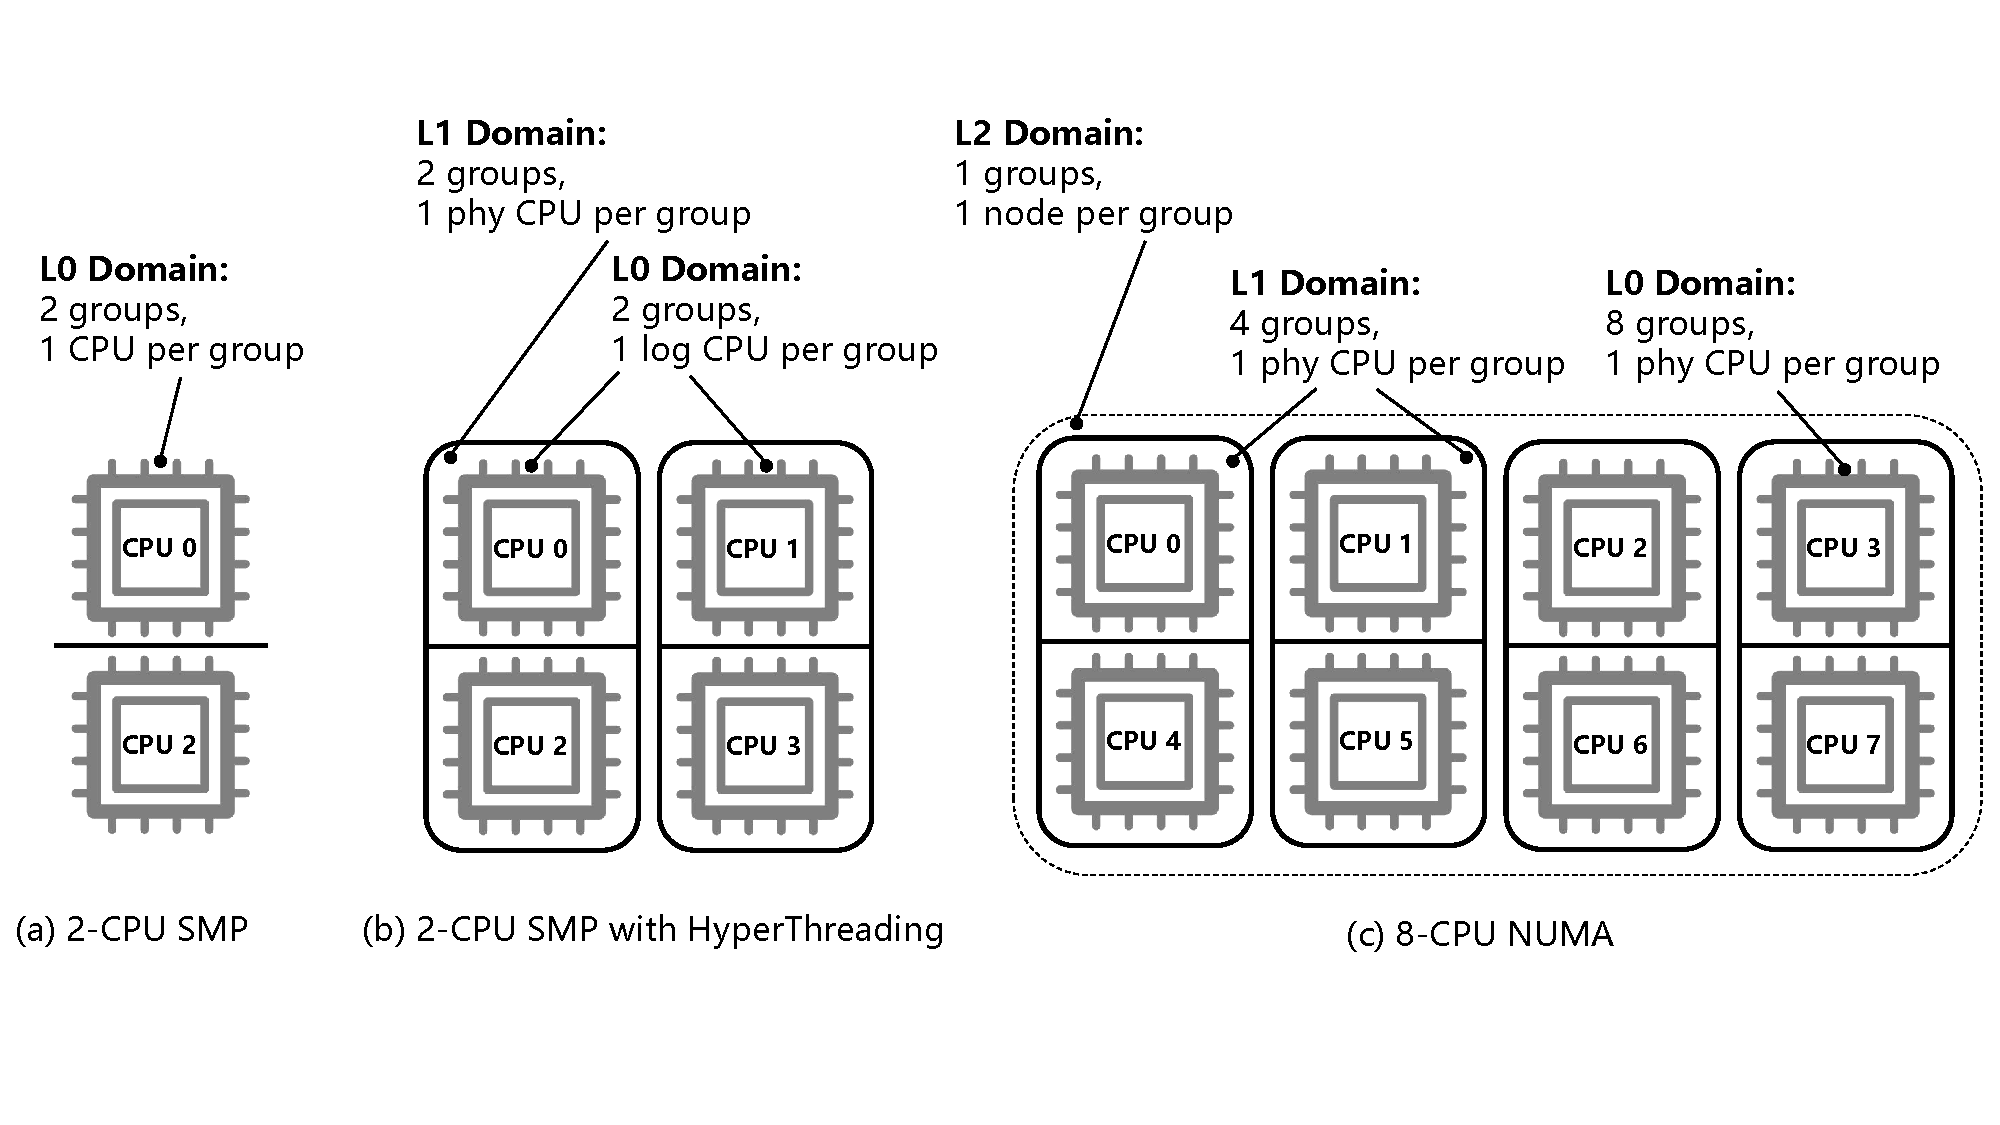
\includegraphics[width=0.80\textwidth]{scheduling_domain}
    \bicaption{\quad 调度域层级}{\quad examples of scheduling domain hierachies}
    \label{fig:scheduling_domain}
\end{figure}


调度域充分反映了以CPU为核心的资源共享信息。








\section{国内外相关研究}

% 可观测性技术用来进行应用画像与劣化监测
% - 谁和谁能够混部
%   - 人为优先级: 延迟(LC/BE)
%   - 资源使用倾向/敏感度
% - 目标应用是否出现性能劣化/资源极限
% 调度技术的划分方式:
% - 实质: 
%   - CPU数量远小于任务数量时, 分时复用是常态,调度主要面向任务切换
%   - CPU数量足够时,任务可以并行,此时资源(异构CPU\Cache\Memory\IO\Net)共享是常态,因此调度主要面向资源划分
% - 任务切换: 修改或定制任务切换的逻辑,通过分时复用来实现共享资源的假象
%   - 实质是创建时间隔离域,来规避竞争
%   - 切换粒度与调度效果强相关, 能否及时响应任务的调度需求是设计的目标
% - 资源划分: 对任务使用的资源进行限制
%    - 创建资源隔离域,来规避竞争
%   - 任务仍在运行|任务由内核进行调度|不干涉任务调度过程
% 调度策略的划分方式:
% - 任务调度: 集中式、工作窃取、FIFO、CFS、EEVDF
% - 资源划分: 资源拆借

\subsection{数据中心可观测性技术研究现状}

劣化监测

分布式追踪(简单提一下)

\subsection{基于资源分配的SLO保障研究现状}

常规

细粒度

\subsection{基于任务调度的SLO保障研究现状}

Linux内核

微秒级调度

\section{论文的研究内容}

\subsection{典型应用画像与混部分析}

\subsection{运行时可变调度框架实现}

\subsection{资源感知调度系统实现}

\section{论文结构安排}
